\chapter{Cadre du projet}

\section{Introduction}
Au début de ce chapitre, le contexte global du projet est posé. On part avec une présentation de l’organisme d’accueil, suivi par ses prestations ainsi que les outils technologiques utilisés. Plutôt que de rester vague, on examine ici comment notre approche se distingue des systèmes préexistants. Petit à petit, la manière choisie pour concevoir le système prend forme. L’intention ? Offrir un tour complet dès le départ : comprendre qui accueille, voir ce qui existe déjà, puis cerner précisément les attentes techniques comme celles hors technique.

\FloatBarrier % Force toutes les images précédentes à être placées
\section{Contexte général du projet}

\subsection{Cadre du projet}
Ce stage donne une chance rare d’aller plus loin que les cours, tout en mettant les pieds dans la réalité du travail en informatique. Pour valider notre formation d’ingénieur en Génie Logiciel, on a rejoint l’équipe de VisioAd. L'idée ? Créer un outil utile, pas juste théorique : une appli CRM appelée « W261 - CRM Micro-SaaS », pensée pour des commerciaux B2B. Elle doit surtout tenir la route quand le volume monte - rapide, souple, bien construite.

\subsection{Présentation de la société d'accueil : VisioAd}
VisioAd est une entreprise innovante spécialisée dans le développement de solutions digitales pour le marketing et la gestion commerciale. Fondée en 2021, elle accompagne les entreprises dans leur transformation numérique grâce à des outils performants d'analyse de données, d'automatisation marketing et de gestion de campagnes publicitaires.

\begin{figure}[!htbp]
    \centering
    
\includegraphics[width=0.7\textwidth,height=0.35\textheight,keepaspectratio]{images/logo-visioad.jpg}
    \caption{Logo de VisioAd}
    \label{fig:logo-visioad}
\end{figure}
\FloatBarrier % Force cette image à être placée ici

VisioAd opère à l'échelle internationale avec des bureaux en Europe et en Amérique du Nord. L'entreprise valorise l'innovation, la qualité technique et l'expérience utilisateur, ce qui en fait un partenaire idéal pour le développement d'un CRM moderne.

\subsubsection{Services}
VisioAd offre une gamme de services adaptés aux besoins numériques des entreprises :
\begin{itemize}
    \item \textbf{Développement d'applications sur mesure} : solutions web et mobiles.
    \item \textbf{Automatisation marketing} : outils de gestion de campagnes et d'analyse comportementale.
    \item \textbf{Business Intelligence} : tableaux de bord interactifs et rapports personnalisés.
    \item \textbf{Conseil en transformation numérique} : accompagnement stratégique et technique.
\end{itemize}

\subsubsection{Technologies adoptées}
VisioAd utilise un stack technologique moderne et varié :
\begin{itemize}
    \item \textbf{Front-end} : React, Next.js, TypeScript, Tailwind CSS
    \item \textbf{Back-end} : Node.js, NestJS, Python, Go
    \item \textbf{Bases de données} : PostgreSQL, MongoDB, Redis
    \item \textbf{Cloud \& DevOps} : AWS, Docker, Kubernetes, CI/CD (GitHub Actions)
    \item \textbf{Analytics} : Tableau, Power BI, intégrations API
\end{itemize}

\FloatBarrier
\section{Idée émergeante et étude de l'existant}

\subsection{Idée émergeante}
Consciente des défis rencontrés par les petites et moyennes équipes B2B dans la gestion de leurs leads et pipelines, VisioAd a initié le développement d'un CRM léger, performant et facile à prendre en main. L'objectif est de combler le fossé entre les solutions CRM complexes et coûteuses et les outils basiques qui manquent de fonctionnalités avancées.

\begin{figure}[!htbp]
    \centering
    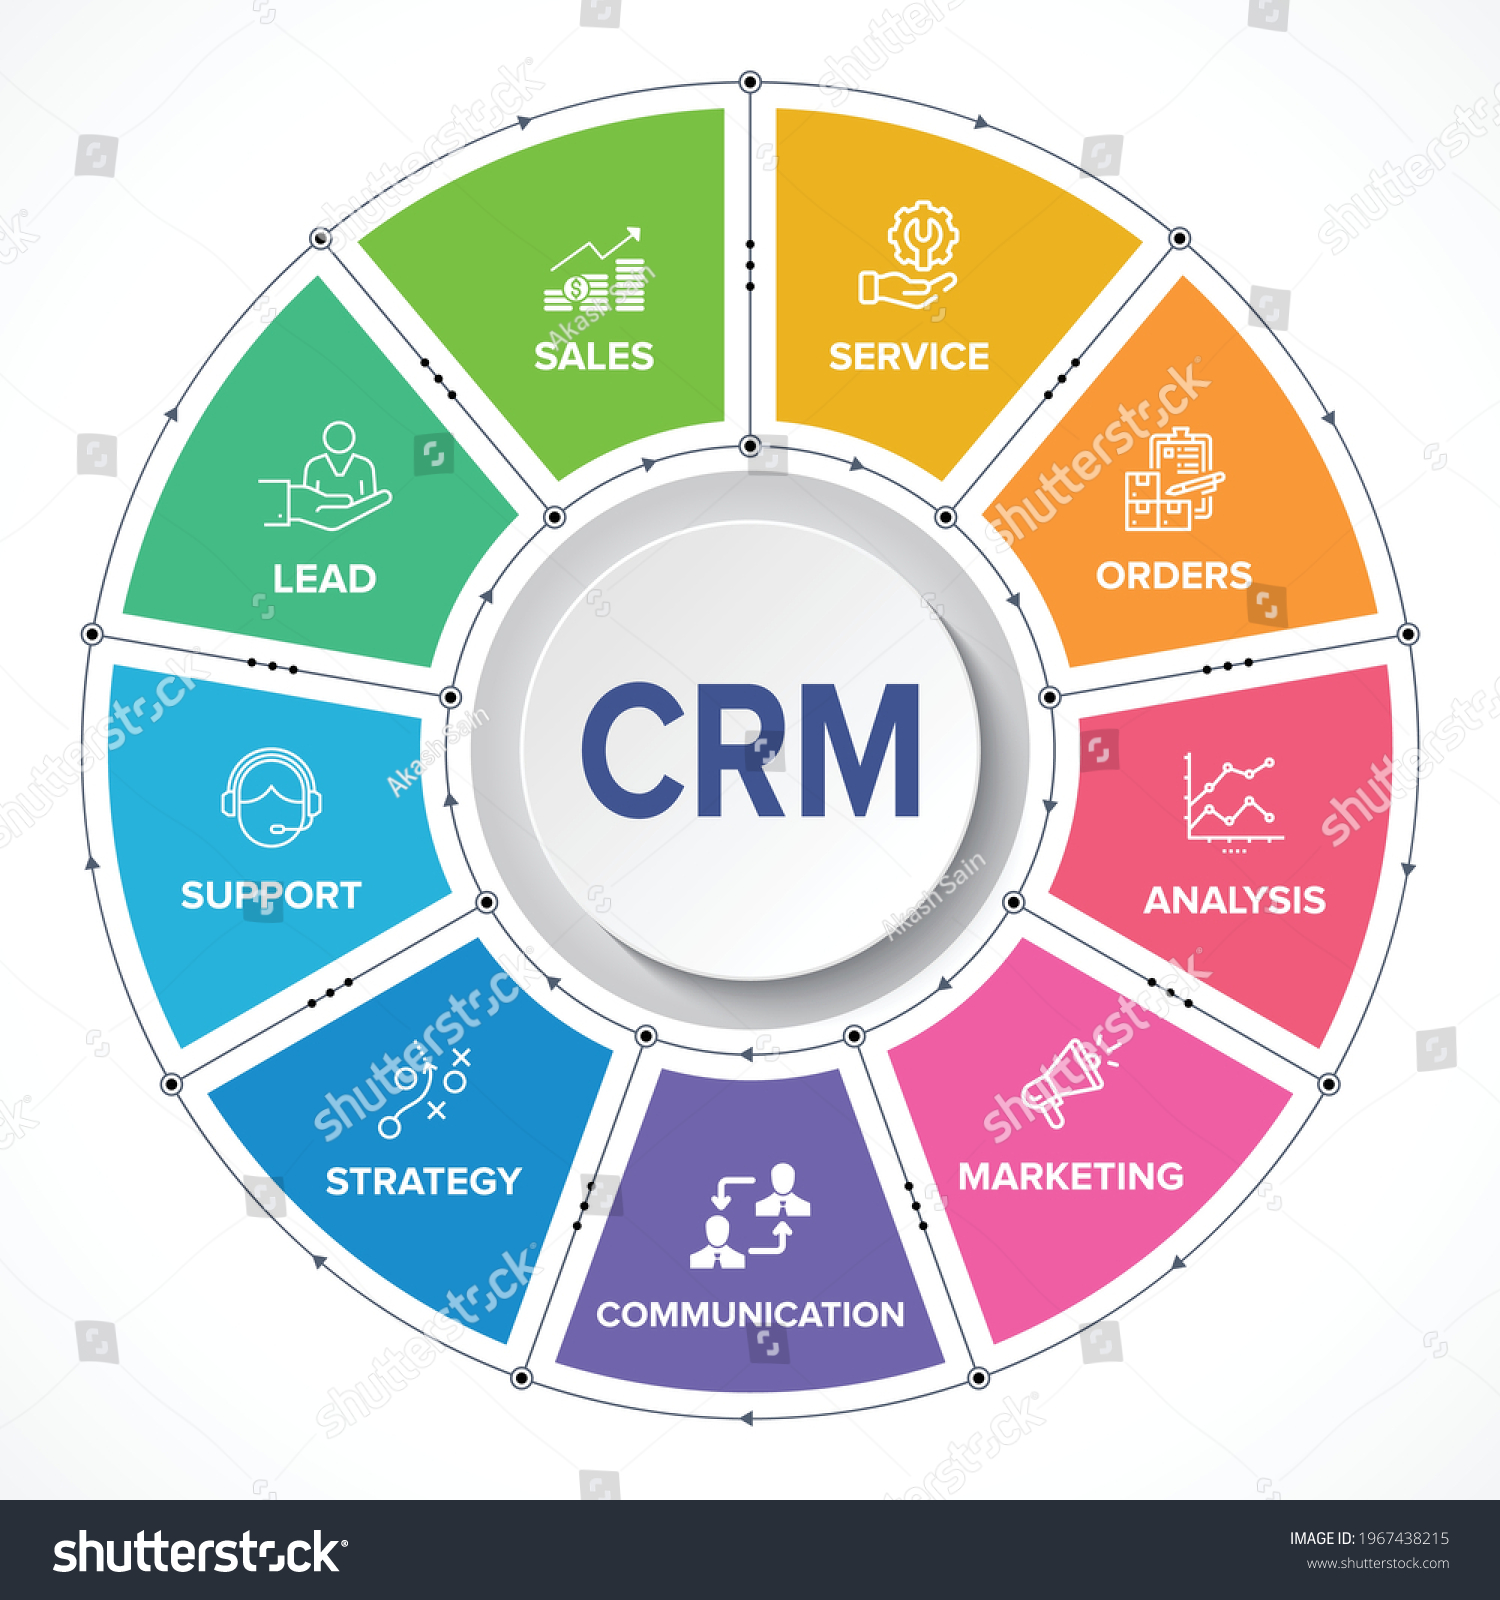
\includegraphics[width=\textwidth,height=0.82\textheight,keepaspectratio]{images/schema-crm-concept.jpg}
    \caption{Architecture conceptuelle du CRM}
    \label{fig:schema-crm}
\end{figure}
\FloatBarrier

\subsection{Analyse comparative des CRM existants}
Une analyse approfondie des trois principales solutions CRM du marché a été réalisée pour identifier leurs forces et faiblesses, et ainsi mieux positionner notre solution.

\subsubsection{Salesforce CRM}
Salesforce est la solution CRM leader du marché, offrant une plateforme complète pour les grandes entreprises.

\begin{figure}[!htbp]
    \centering
    
\includegraphics[width=0.8\textwidth,height=0.45\textheight,keepaspectratio]{images/Salesforce Logo.jpg}
    \caption{Interface de Salesforce CRM}
    \label{fig:salesforce}
\end{figure}
\FloatBarrier

\textbf{Avantages :}
\begin{itemize}
    \item Fonctionnalités très complètes
    \item Écosystème d'applications étendu
    \item intégrations avec de nombreuses plateformes
\end{itemize}

\textbf{Limites :}
\begin{itemize}
    \item Coût très élevé
    \item Complexité de configuration
    \item Surdimensionné pour les petites équipes
\end{itemize}

\textbf{Avantage de notre solution :} Notre CRM offre une alternative abordable et simplifiée, spécialement conçue pour les petites équipes B2B, avec une courbe d'apprentissage réduite.

\subsubsection{HubSpot CRM}
HubSpot propose une solution CRM gratuite avec des options payantes pour les fonctionnalités avancées.

\begin{figure}[!htbp]
    \centering
    
\includegraphics[width=0.8\textwidth,height=0.45\textheight,keepaspectratio]{images/HubSpot-Logo.png}
    \caption{Interface de HubSpot CRM}
    \label{fig:hubspot}
\end{figure}
\FloatBarrier

\textbf{Avantages :}
\begin{itemize}
    \item Version gratuite disponible
    \item Interface utilisateur intuitive
    \item Bonnes intégrations marketing
\end{itemize}

\textbf{Limites :}
\begin{itemize}
    \item Fonctionnalités limitées dans la version gratuite
    \item Personnalisation restreinte
    \item Performances moyennes avec grands volumes
\end{itemize}

\textbf{Avantage de notre solution :} Notre CRM offre une personnalisation complète sans limitations artificielles, avec des performances optimisées pour traiter des milliers de leads sans ralentissement.

\subsubsection{Zoho CRM}
Zoho CRM est une solution flexible adaptée aux entreprises de différentes tailles.

\begin{figure}[!htbp]
    \centering
    
\includegraphics[width=0.8\textwidth,height=0.45\textheight,keepaspectratio]{images/zoho-logo-512.png}
    \caption{Interface de Zoho CRM}
    \label{fig:zoho}
\end{figure}
\FloatBarrier

\textbf{Avantages :}
\begin{itemize}
    \item Coût raisonnable
    \item Bonne personnalisation
    \item Suite d'outils intégrés
\end{itemize}

\textbf{Limites :}
\begin{itemize}
    \item Interface parfois complexe
    \item Performances limitées pour les grands volumes
    \item Expérience utilisateur inégale
\end{itemize}

\textbf{Avantage de notre solution :} Notre CRM utilise une architecture moderne avec virtualisation des données, garantissant une interface fluide même avec 10 000+ leads, et une expérience utilisateur cohérente.

\subsection{Tableau comparatif synthétique}

\begin{table}[!htbp]
\centering
\caption{Comparaison des CRM existants avec notre solution}
\label{tab:comparaison-crm}
\begin{tabular}{|p{3cm}|p{2.5cm}|p{2.5cm}|p{2.5cm}|p{2.5cm}|}
\hline
\textbf{Critère} & \textbf{Salesforce} & \textbf{HubSpot} & \textbf{Zoho} & \textbf{Notre CRM} \\
\hline
Coût & Très élevé & Modéré/Gratuit & Raisonnable & Abordable \\
\hline
Complexité & Élevée & Moyenne & Moyenne-élevée & Faible \\
\hline
Personnalisation & Avancée & Limitée & Bonne & Complète \\
\hline
Performance grands volumes & Bonne & Moyenne & Limitée & Excellente \\
\hline
Interface & Professionnelle & Intuitive & Inégale & Moderne/Fluide \\
\hline
Spécialisation B2B & Générale & Marketing & Générale & Spécifique B2B \\
\hline
\end{tabular}
\end{table}
\FloatBarrier

\begin{figure}[!htbp]
    \centering
    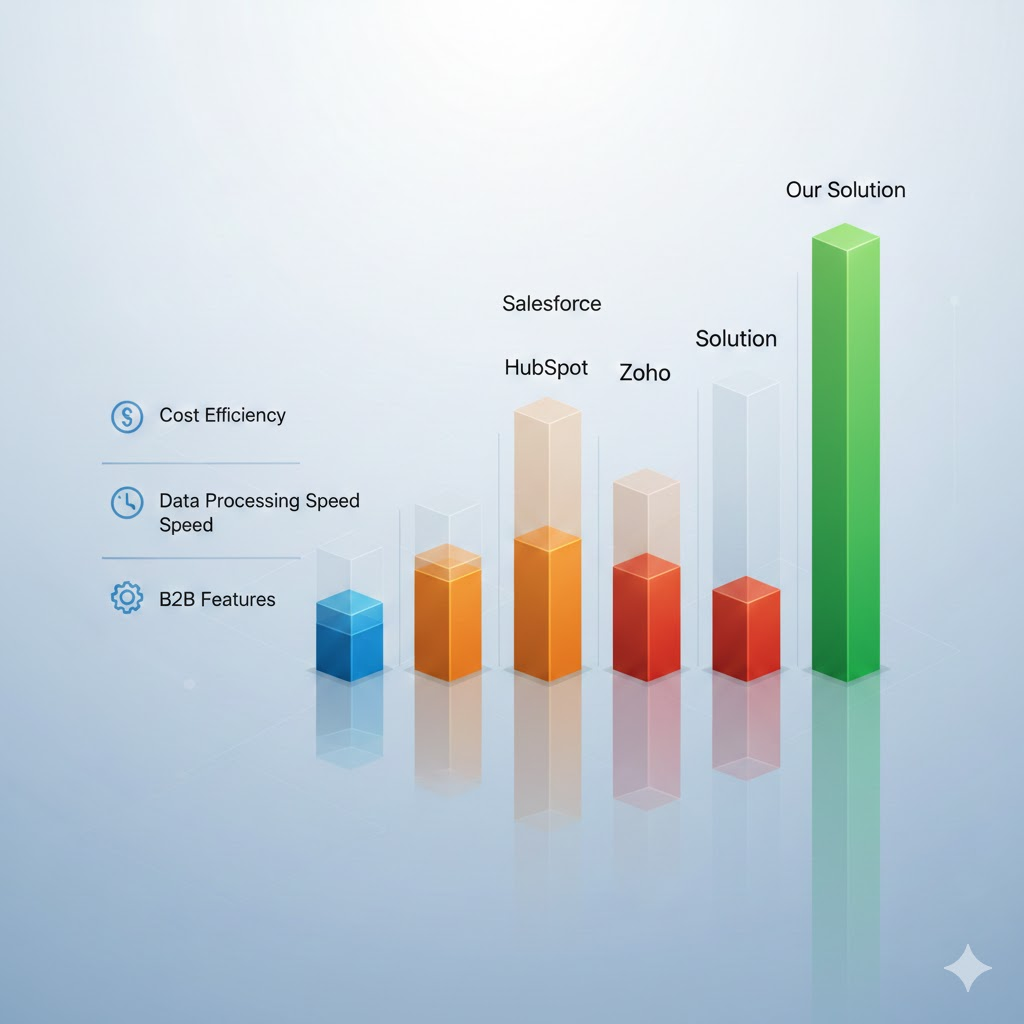
\includegraphics[width=\textwidth,height=0.82\textheight,keepaspectratio]{images/comparaison.jpg}
    \caption{Visualisation comparative des différents CRM}
    \label{fig:comparaison-graphique}
\end{figure}
\FloatBarrier

\subsection{Critique de l'existant}

\subsubsection{Critique du système actuel}
Les solutions CRM actuelles présentent plusieurs limites :
\begin{itemize}
    \item Complexité de configuration et de déploiement.
    \item Coût élevé pour les petites équipes.
    \item Performances dégradées avec de grands volumes de données.
    \item Manque de personnalisation fine pour les workflows B2B.
\end{itemize}

\subsubsection{État de l'art}
Pour proposer une solution compétitive, nous avons étudié des approches modernes de gestion de données volumineuses et d'optimisation d'interface, notamment :
\begin{itemize}
    \item Virtualisation des tableaux de données (TanStack Table).
    \item Architecture serverless et microservices.
    \item Traitement par lots (batch processing) pour l'import CSV.
\end{itemize}

\begin{figure}[!htbp]
    \centering
    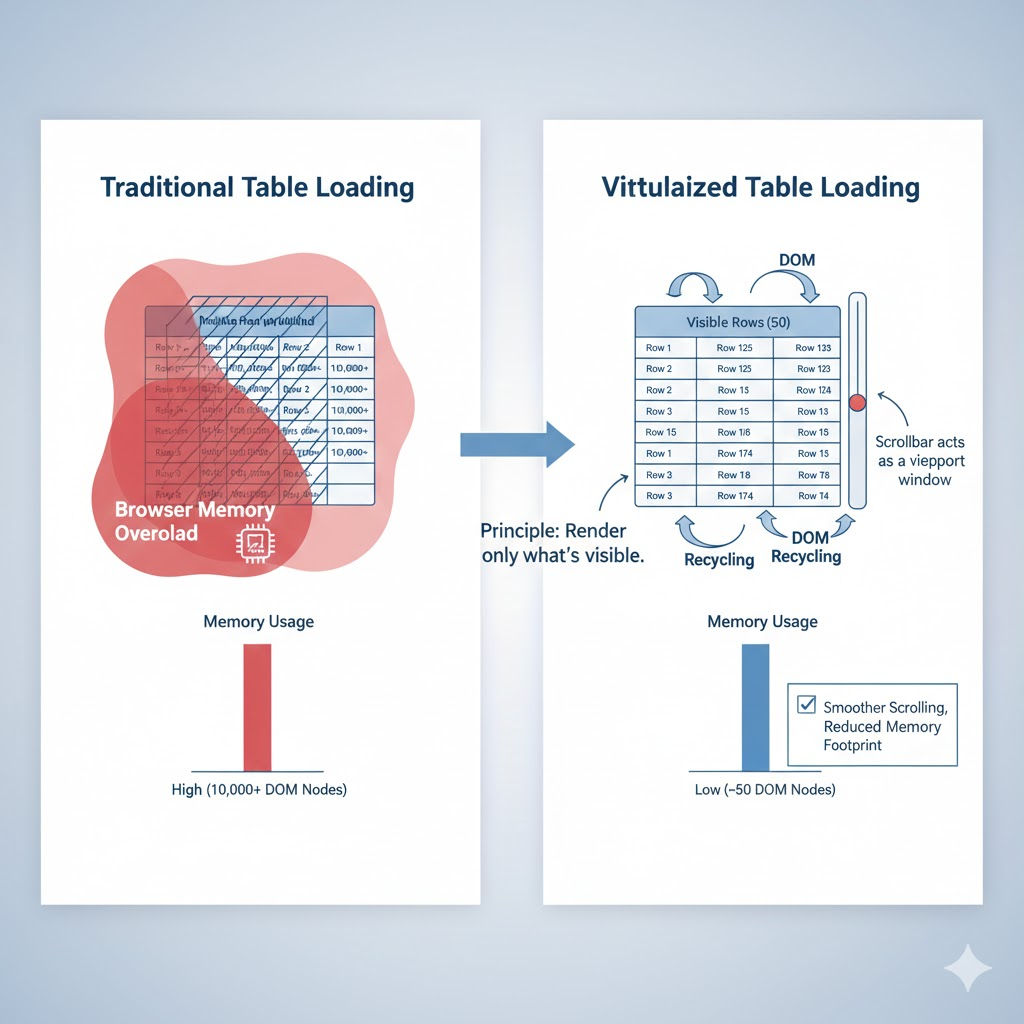
\includegraphics[width=\textwidth,height=0.82\textheight,keepaspectratio]{images/etat.jpg}
    \caption{Principe de virtualisation dans les interfaces data-grid}
    \label{fig:virtualisation}
\end{figure}
\FloatBarrier

\subsection{Solution proposée}
Nous proposons un CRM Micro-SaaS axé sur :
\begin{itemize}
    \item \textbf{Performance} : Interface fluide même avec des milliers d'enregistrements grâce à la virtualisation.
    \item \textbf{Simplicité} : Pipeline de vente modulable et visuel, facile à configurer.
    \item \textbf{Productivité} : Intégration native d'import CSV avec mapping intelligent.
    \item \textbf{Analyse} : Tableau de bord analytique en temps réel.
    \item \textbf{Scalabilité} : Architecture moderne et scalable.
\end{itemize}

\begin{figure}[!htbp]
    \centering
    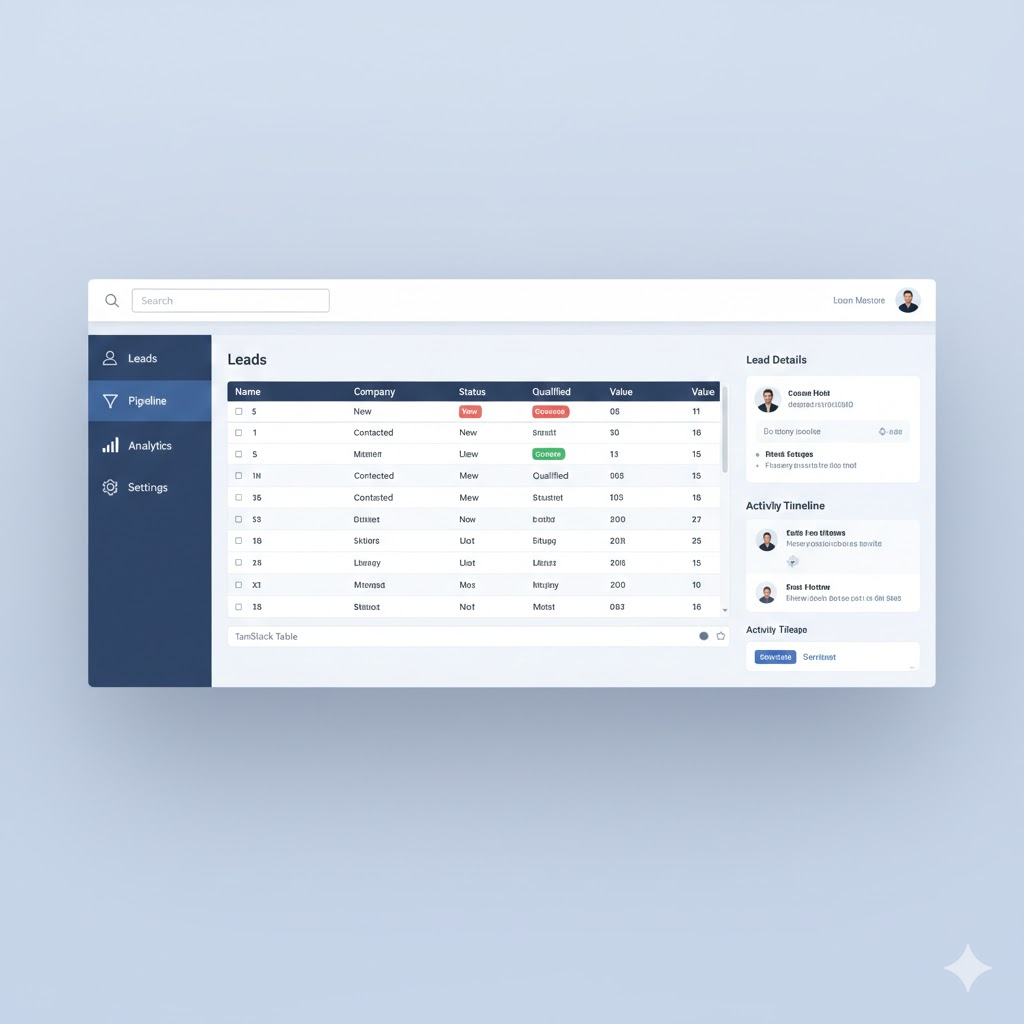
\includegraphics[width=\textwidth,height=0.82\textheight,keepaspectratio]{images/concept.jpg}
    \caption{Aperçu de notre solution CRM}
    \label{fig:notre-solution}
\end{figure}
\FloatBarrier

\section{Méthodologie de développement}

\subsection{Étude des méthodes existantes}
\label{sec:etude-methodes}
Plusieurs méthodologies de développement ont été étudiées pour choisir celle la plus adaptée à un projet agile et technique :

\subsubsection{Scrum}
Scrum est une méthode agile itérative et incrémentale, idéale pour les projets nécessitant une forte adaptabilité. Elle se caractérise par des sprints courts (2-4 semaines), des rituels réguliers (daily stand-up, sprint planning, review, retrospective) et une forte collaboration avec le client.

\begin{figure}[!htbp]
    \centering
    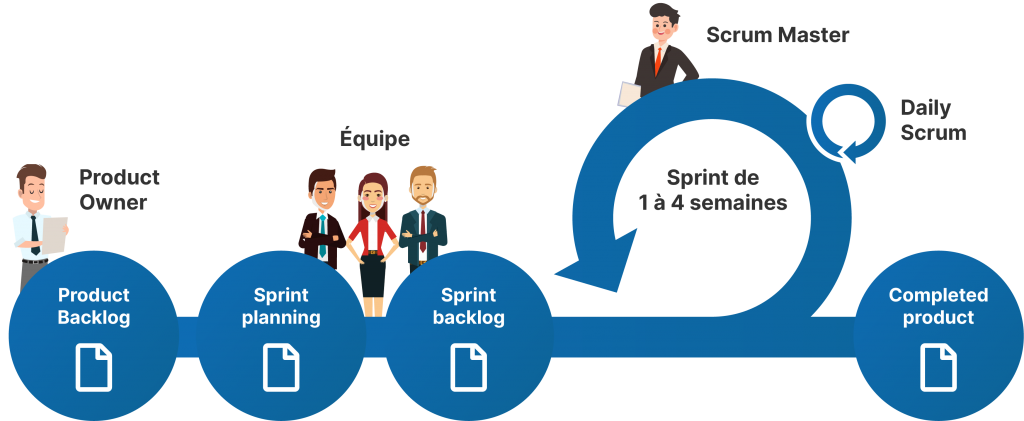
\includegraphics[width=\textwidth,height=0.82\textheight,keepaspectratio]{images/processus-scrum.png}
    \caption{Processus Scrum}
    \label{fig:scrum}
\end{figure}
\FloatBarrier

\subsubsection{Extreme Programming (XP)}
Extreme Programming (XP) met l'accent sur la qualité du code, les tests automatisés et l'intégration continue. Ses valeurs principales sont la simplicité, la communication, le feedback et le courage. XP est particulièrement adaptée aux projets nécessitant une grande flexibilité face aux changements de requirements.

\begin{figure}[!htbp]
    \centering
    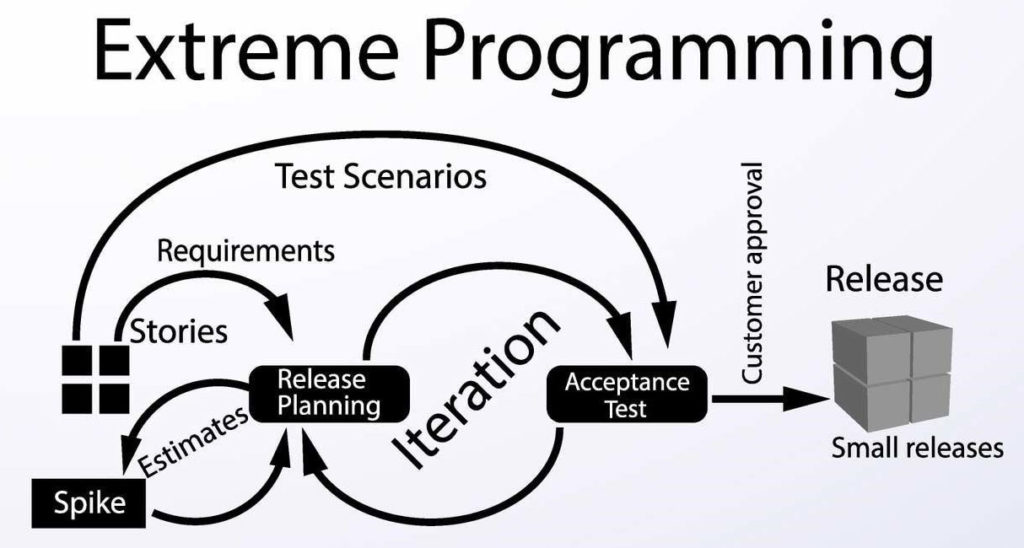
\includegraphics[width=\textwidth,height=0.82\textheight,keepaspectratio]{images/processus-xp.jpeg}
    \caption{Processus Extreme Programming (XP)}
    \label{fig:xp}
\end{figure}
\FloatBarrier

\subsubsection{Kanban}
Kanban permet une visualisation claire du flux de travail et une limitation des tâches en cours. Basée sur le système de production Toyota, cette méthode utilise un tableau avec des colonnes (To Do, In Progress, Done) pour visualiser l'avancement des tâches et identifier les goulots d'étranglement.

\begin{figure}[!htbp]
    \centering
    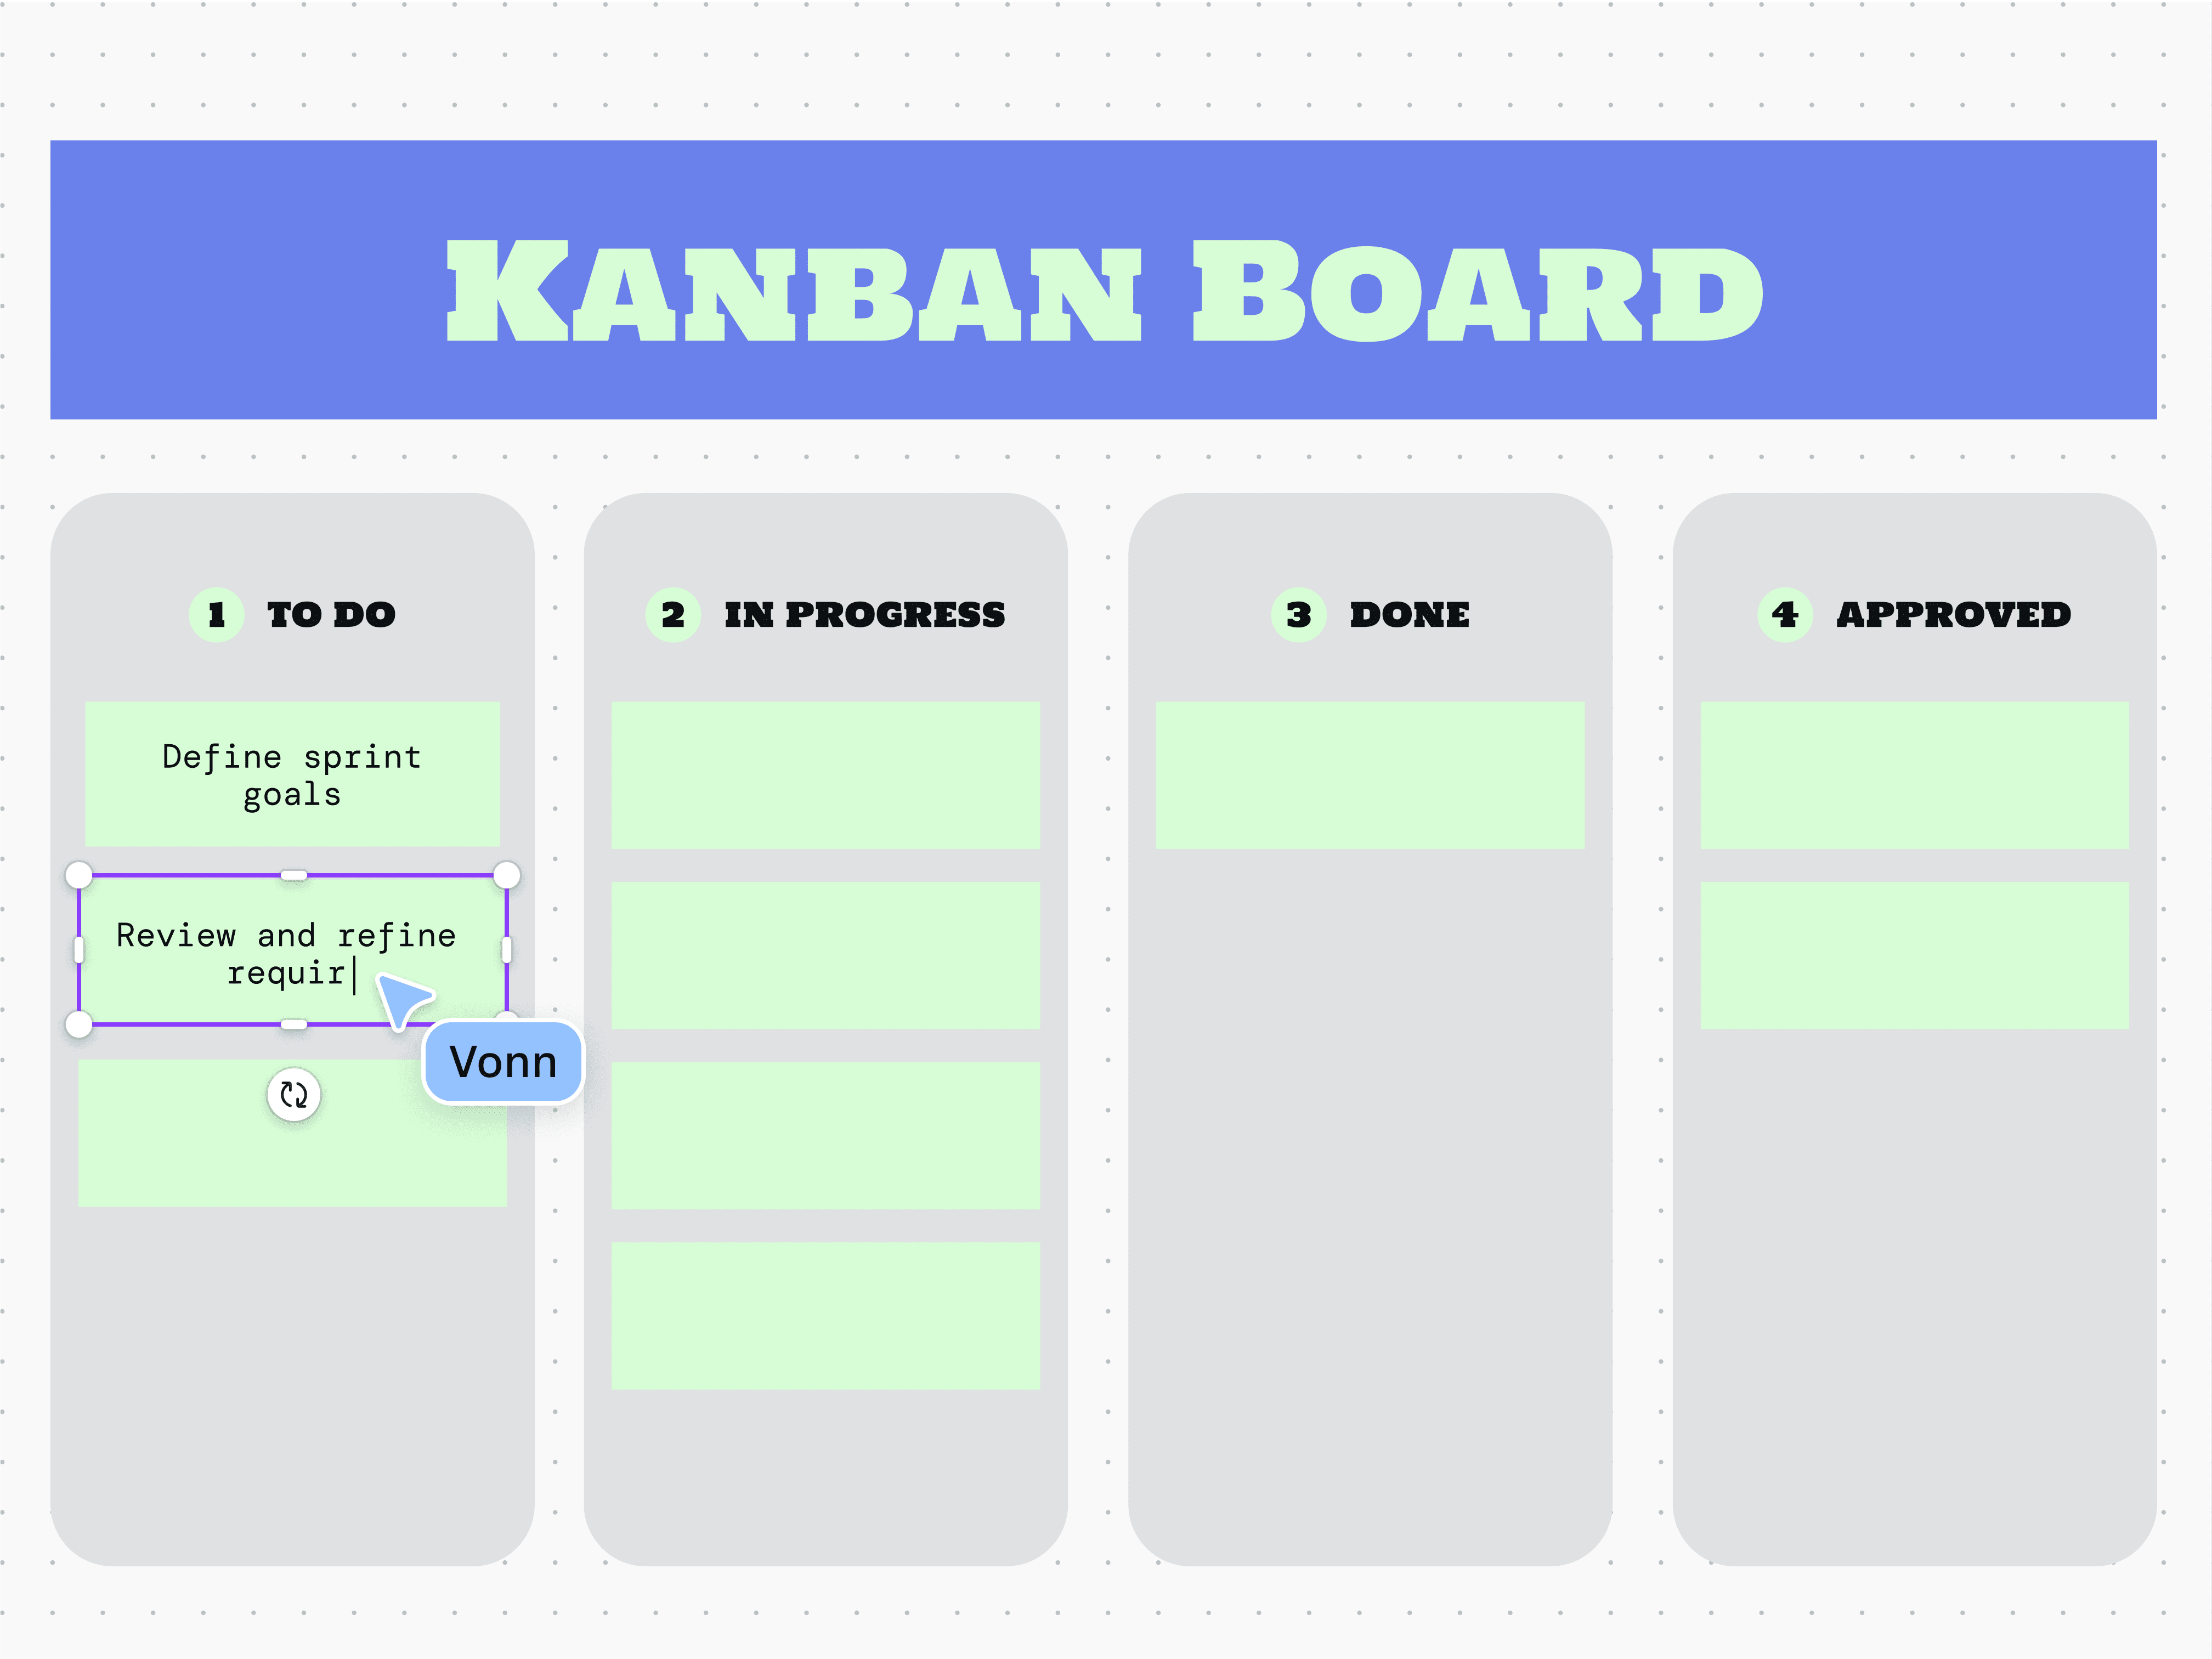
\includegraphics[width=\textwidth,height=0.82\textheight,keepaspectratio]{images/kanban.png}
    \caption{Processus Kanban}
    \label{fig:kanban}
\end{figure}
\FloatBarrier

\subsubsection{Waterfall (Cascade)}
La méthode Waterfall (ou en cascade) suit une approche séquentielle linéaire avec des phases bien définies : Conception, Implémentation, Test, Déploiement, Maintenance. Chaque phase doit être complétée avant de passer à la suivante, ce qui la rend prévisible mais peu flexible.

\begin{figure}[!htbp]
    \centering
    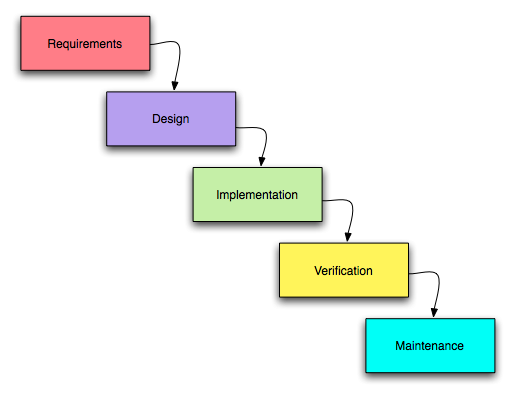
\includegraphics[width=\textwidth,height=0.82\textheight,keepaspectratio]{images/waterfall.png}
    \caption{Processus Waterfall (Cascade)}
    \label{fig:waterfall}
\end{figure}
\FloatBarrier

\subsubsection{Unified Process (UP)}
Unified Process est une méthodologie itérative et incrémentale qui combine des éléments des méthodes agiles et traditionnelles. Elle se décompose en quatre phases : Inception, Elaboration, Construction, Transition.

\begin{figure}[!htbp]
    \centering
    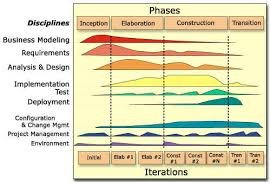
\includegraphics[width=\textwidth,height=0.82\textheight,keepaspectratio]{images/up.jpg}
    \caption{Processus Unified Process (UP)}
    \label{fig:up}
\end{figure}
\FloatBarrier

\subsubsection{Two-Track Unified Process (2TUP)}
2TUP est une variante d'UP qui sépare le développement en deux pistes parallèles : une piste fonctionnelle (métier) et une piste technique (architecture). Cette séparation permet une meilleure gestion des changements et une plus grande flexibilité.

\begin{figure}[!htbp]
    \centering
    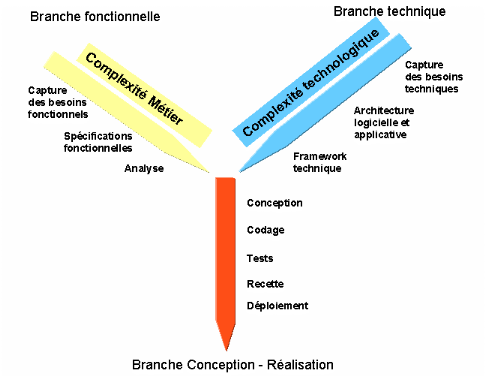
\includegraphics[width=\textwidth,height=0.82\textheight,keepaspectratio]{images/tup.png}
    \caption{Processus Two-Track Unified Process (2TUP)}
    \label{fig:2tup}
\end{figure}
\FloatBarrier

\subsection{Choix de la méthodologie}
Après analyse des différentes méthodes présentées dans la section \ref{sec:etude-methodes}, nous avons opté pour la méthodologie \textbf{2TUP} (Two-Track Unified Process) comme processus de développement principal pour notre projet CRM Micro-SaaS.

\subsubsection{Raisons du choix de 2TUP}
Le choix de 2TUP repose sur plusieurs raisons fondamentales qui correspondent parfaitement aux contraintes et aux objectifs de notre projet :

\begin{enumerate}
    \item \textbf{Séparation claire entre la branche fonctionnelle et la branche technique :}
    Notre projet CRM comporte deux dimensions très distinctes. D'un côté, une \textit{branche fonctionnelle} riche (gestion des leads, pipeline commercial, tickets de support, génération d'emails par IA, scoring prédictif) qui nécessite une analyse métier approfondie. De l'autre, une \textit{branche technique} complexe (architecture micro-services, intégration d'API externes comme Google Gemini et FastAPI, conteneurisation Docker/Kubernetes, ORM Prisma). 2TUP permet de mener ces deux pistes en parallèle avant de les fusionner lors de la phase de conception, ce qui est idéal pour notre contexte.

    \item \textbf{Approche itérative et incrémentale adaptée aux sprints du projet :}
    2TUP suit un cycle de vie itératif et incrémental, ce qui s'aligne directement avec notre planification en \textbf{4 sprints} successifs (Conception \& BDD, API \& Frontend, UI \& Tests, Documentation \& Soutenance). Chaque sprint produit un livrable fonctionnel et testable, permettant une validation progressive du système.

    \item \textbf{Compatibilité native avec le formalisme UML :}
    2TUP, en tant que variante du Unified Process, s'appuie nativement sur le langage de modélisation \textbf{UML} pour la spécification, la conception et la documentation. Cela garantit une cohérence totale entre notre méthodologie et nos livrables de modélisation (diagrammes de cas d'utilisation, de séquence, de classes et de déploiement).

    \item \textbf{Gestion maîtrisée des risques techniques :}
    L'intégration de services d'intelligence artificielle (API Gemini, micro-service de scoring) introduit des risques techniques importants (latence réseau, indisponibilité des API, qualité des prédictions). La branche technique de 2TUP permet d'identifier et de traiter ces risques architecturaux dès les premières phases, notamment à travers les mécanismes de \textit{fallback} (Graceful Degradation) que nous avons mis en place.

    \item \textbf{Flexibilité face aux changements de spécifications :}
    Dans le cadre d'un projet de fin d'études réalisé au sein d'une entreprise (VisioAd), les exigences peuvent évoluer en cours de développement. Contrairement à la méthode Waterfall qui fige les spécifications, 2TUP offre une souplesse d'adaptation grâce à ses itérations successives, tout en conservant une rigueur de documentation supérieure aux méthodes purement agiles.
\end{enumerate}

\begin{figure}[!htbp]
    \centering
    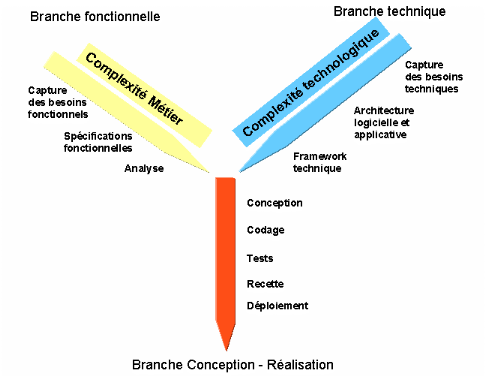
\includegraphics[width=\textwidth,height=0.82\textheight,keepaspectratio]{images/tup.png}
    \caption{Processus 2TUP adopté pour le projet CRM}
    \label{fig:methode-2tup-choix}
\end{figure}
\FloatBarrier

\subsection{Choix des formalismes adéquats}
Pour la modélisation et la documentation de notre système, nous avons adopté le langage \textbf{UML} (Unified Modeling Language) comme formalisme de référence. Ce choix se justifie par les raisons suivantes :

\begin{itemize}
    \item \textbf{Standard universel :} UML est le langage de modélisation le plus répandu dans l'industrie du génie logiciel, ce qui facilite la communication entre les parties prenantes du projet.
    \item \textbf{Cohérence avec 2TUP :} Le processus 2TUP repose intrinsèquement sur les diagrammes UML pour formaliser les résultats de chaque phase (branche fonctionnelle et branche technique).
    \item \textbf{Couverture complète :} UML offre une palette de diagrammes couvrant tous les aspects de notre système :
    \begin{itemize}
        \item \textit{Diagrammes de cas d'utilisation} pour capturer les besoins fonctionnels par acteur.
        \item \textit{Diagrammes de séquence système} pour modéliser les interactions temporelles entre les composants (Frontend, Backend, API IA).
        \item \textit{Diagramme de classes} pour structurer le modèle de données et les relations entre entités.
        \item \textit{Diagramme de déploiement} pour représenter l'architecture physique micro-services (Next.js, NestJS, FastAPI, MySQL, Docker).
    \end{itemize}
    \item \textbf{Outil de documentation pérenne :} Les diagrammes UML constituent une documentation technique durable, facilitant la maintenance et l'évolution future du CRM.
\end{itemize}

\section{Planification}
Au départ, on a dessiné un graphique pour voir comment se passe le travail. Chaque étape importante apparaît dedans, avec des dates étalées de février à juillet. Grâce à ce repère visuel, il est plus simple de mesurer où en est le chantier. Quelque chose change ? On réorganise sans tarder selon les besoins du moment.

\begin{figure}[!htbp]
    \centering
    \resizebox{\textwidth}{!}{
    \renewcommand{\arraystretch}{1.5} % Espace entre les lignes
    \begin{tabular}{|p{7.5cm}|*{16}{c|}}
    \hline
    \rowcolor{gray!70}
    \textbf{\textcolor{white}{Tâches / User Stories}} & 
    \multicolumn{4}{c|}{\cellcolor{blue!70}\textbf{\textcolor{white}{Incrément 1 : Conception \& BDD}}} & 
    \multicolumn{4}{c|}{\cellcolor{red!70}\textbf{\textcolor{white}{Incrément 2 : API \& Frontend}}} & 
    \multicolumn{4}{c|}{\cellcolor{orange!70}\textbf{\textcolor{white}{Incrément 3 : UI \& Tests}}} & 
    \multicolumn{4}{c|}{\cellcolor{green!70}\textbf{\textcolor{white}{Incrément 4 : Doc \& Soutenance}}} \\
    \hline
    \rowcolor{gray!20}
    \textbf{Période $\rightarrow$ Sem.} & 
    \textbf{S1} & \textbf{S2} & \textbf{S3} & \textbf{S4} & 
    \textbf{S5} & \textbf{S6} & \textbf{S7} & \textbf{S8} & 
    \textbf{S9} & \textbf{S10} & \textbf{S11} & \textbf{S12} & 
    \textbf{S13} & \textbf{S14} & \textbf{S15} & \textbf{S16} \\
    \hline
    
    % SPRINT 1
    \multicolumn{17}{|l|}{\cellcolor{gray!10}\textbf{SPRINT 1 TASKS}} \\
    \hline
    US-01 : Analyse des besoins et conception & \cellcolor{blue!50} & \cellcolor{blue!50} & & & & & & & & & & & & & & \\
    \hline
    US-02 : Développement de la base de données & & & \cellcolor{blue!50} & \cellcolor{blue!50} & & & & & & & & & & & & \\
    \hline
    
    % SPRINT 2
    \multicolumn{17}{|l|}{\cellcolor{gray!10}\textbf{SPRINT 2 TASKS}} \\
    \hline
    US-03 : Développement de l'API backend & & & & & \cellcolor{red!50} & \cellcolor{red!50} & & & & & & & & & & \\
    \hline
    US-04 : Développement du frontend (Interface) & & & & & & & \cellcolor{red!50} & \cellcolor{red!50} & & & & & & & & \\
    \hline
    
    % SPRINT 3
    \multicolumn{17}{|l|}{\cellcolor{gray!10}\textbf{SPRINT 3 TASKS}} \\
    \hline
    US-05 : Développement frontend (Virtualisation) & & & & & & & & & \cellcolor{orange!50} & \cellcolor{orange!50} & & & & & & \\
    \hline
    US-06 : Tests et optimisation des performances & & & & & & & & & & & \cellcolor{orange!50} & \cellcolor{orange!50} & & & & \\
    \hline
    
    % SPRINT 4
    \multicolumn{17}{|l|}{\cellcolor{gray!10}\textbf{SPRINT 4 TASKS}} \\
    \hline
    US-07 : Documentation et préparation démo & & & & & & & & & & & & & \cellcolor{green!50} & \cellcolor{green!50} & & \\
    \hline
    US-08 : Soutenance et livraison finale & & & & & & & & & & & & & & & \cellcolor{green!50} & \cellcolor{green!50} \\
    \hline
    
    % Timeline du bas
    \rowcolor{gray!20}
    \textbf{Mois} & \multicolumn{4}{c|}{\textbf{Février - Mars 2026}} & \multicolumn{4}{c|}{\textbf{Avril - Mai 2026}} & \multicolumn{4}{c|}{\textbf{Juin 2026}} & \multicolumn{4}{c|}{\textbf{Juillet 2026 (Soutenance)}} \\
    \hline
    \end{tabular}
    }
    \caption{Diagramme de Gantt du projet CRM (Février à Juillet - 4 Incréments)}
    \label{fig:gantt}
\end{figure}
\FloatBarrier

Les principales phases du projet sont :
\begin{itemize}
    \item \textbf{Semaines 1-2} : Analyse des besoins et conception initiale
    \item \textbf{Semaines 3-6} : Développement du backend (API, base de données)
    \item \textbf{Semaines 7-10} : Développement du frontend (interface, virtualisation)
    \item \textbf{Semaines 11-12} : Tests et optimisation des performances
    \item \textbf{Semaines 13-14} : Documentation et préparation de la démonstration
    \item \textbf{Semaines 15-16} : Revue finale et corrections
\end{itemize}

\section{Conclusion}
Dans ce chapitre, nous avons posé le cadre général du projet en commençant par la présentation de l'organisme d'accueil VisioAd et de ses activités. Ensuite, une étude comparative approfondie des CRM existants sur le marché — Salesforce, HubSpot et Zoho — a permis d'identifier leurs forces et leurs limites, et de positionner notre solution comme une alternative adaptée aux petites équipes B2B. Après un examen des méthodologies de développement existantes, notre choix s'est porté sur le processus \textbf{2TUP} (Two-Track Unified Process), dont la séparation en branche fonctionnelle et branche technique correspond idéalement à la double nature de notre projet. Le formalisme \textbf{UML} a été retenu pour la modélisation, en parfaite cohérence avec 2TUP. Enfin, la planification a été structurée en quatre sprints répartis sur seize semaines, de février à juillet 2026, permettant une livraison progressive et maîtrisée du système. Le chapitre suivant se consacrera à l'analyse et à la spécification détaillée des besoins fonctionnels et non fonctionnels.
